
% Szkielet dla pracy pisanej w języku polskim.

\documentclass[polish,a4paper,oneside]{ppfcmthesis}
\usepackage[utf8]{inputenc}
\usepackage[OT4]{fontenc}


\authortitle{inż.~}                                        % You can place "inż.~" here, if you really want to.
\author{Tomasz Kujawa}                              % Your name comes here
\title{Równoległe odkrywanie reguł asocjacyjnyh zaimplementowane na procesory graficzne}                   % Note how we protect the final title phrase from breaking
\ppsupervisor{dr ~inż.~Witold Andrzejwski} % Your supervisor comes here.
\ppyear{2011}                                         % Year of final submission (not graduation!)

\newtheorem{twr}{Twierdzenie}
\newtheorem{lem}[twr]{Lemat}
\newtheorem{df}{Definicja}

\begin{document}

% Front matter starts here
\frontmatter\pagestyle{empty}%
\maketitle\cleardoublepage%

% Blank info page for "karta dyplomowa"
\thispagestyle{empty}\vspace*{\fill}%
\begin{center}Tutaj przychodzi karta pracy dyplomowej;\\oryginał wstawiamy do wersji dla archiwum PP, w pozostałych kopiach wstawiamy ksero.\end{center}%
\vfill\cleardoublepage%

% Table of contents.
\pagenumbering{Roman}\pagestyle{ppfcmthesis}%
\tableofcontents* \cleardoublepage%

% Main content of your thesis starts here.
\mainmatter%
\chapter{Wstęp}
Proces informatyzacji przedsiębiorstw, rozpoczęty kilka dekad temu, wprowadził światową gospodarkę na nowe, dotąd nieznane tory rozwoju. Skrócenie procesu produkcyjnego, wprowadzenie kontroli komputerowych, czy też skomputeryzowanych maszyn skróciło i ułatwiło produkcję,~a~także zarządzanie procesami w firmach i przedsiębiorstwach. Przed ludźmi stanęły możliwości, ale także wyzwania, z~którymi nigdy wcześniej nikt nie musiał sobie radzić. Zmiany, jakie nastąpiły przez ostatnie trzy dekady są nieodwracalne i zmuszają informatyków do tworzenia nowych aplikacji, które będą w stanie sprostać wymaganiom im stawianym.

Informatyzacja firm, instytucji oraz innych jednostek organizacyjnych powinna realizować dwa podstawowe cele. Z~jednej strony powinna ona usprawniać pracę pojedynczego pracownika poprzez automatyzację realizowanych przez niego rutynowych zadań. Dzięki wykorzystaniu możliwości komputerów działania te powinny być wykonywane szybciej i w sposób bardziej niezawodny. Z~drugiej strony celem informatyzacji jest wpływanie na działanie całch firm w wyniku wspomagania decyzji kadry zarządzającej przedsiębiorstwami. Szybka analiza bazująca na pełnej i aktualnej informacji o stanie firmy może ułatwić kadrze zarządzającej podejmowanie trafnych i szybkich decyzje o strategicznym znaczeniu dla rozwoju danego przedsiębiorstwa.

Wprowadzenie komputerów do właściwie każdej przestrzeni ludzkiego życia wpłynęło na wyprodukowanie olbrzymich ilości danych. Reprezentowane są one w sposób umożliwiający ich składowanie i przetwarzanie komputerowe przez aplikacje analityczne. W chwili obecnej ludzkość jest świadkiem eksplozji ilości danych produkowanych przez różnego rodzaju systemy komputerowe. Analiza tych danych przynieść może wymierne korzyści nie tylko w kwestiach finansowych, ale~również poznawczych. Dzięki analizie danych zebranych w przeszłości możliwe jest lepsze dopasowanie planów w przyszłości - na tej podstawie planowane mogą być np. akcje marketingowe, czy~też~promocje w supermarketach spożywczych. Wykorzystanie wiedzy uzyskanej w ten sposób jest niezwykle szerokie i może być użyte w każdym rejonie działalności firmy.

Odkrycie zależności pomiędzy zgromadzonymi danymi bez zastosowania narzędzi informatycznych jest procesem bardzo skomplikowanym i wymagającym do realizacji dużo czasu. Przy obecnej złożoności większości systemów oraz rozmiarom danych produkowanych przez te systemy, kosz czasowy jest na tyle duży, że ręczna analiza tych danych stała się niemożliwa. Dlatego też tworzone są narzędzia umożliwiające odkrywanie prawidłowości w dużych zbiorach danych, by człowiek na tej podstawie mógł podejmować decyzje i wyciągać wnioski.

Dział informatyki, który zajmuje się odkrywaniem ukrytych dla człowieka prawidłowości i reguł w danych nazywa się eksploracją danych (\english{Data Mining}), który jest jednym z etapów procesu \termdef{odkrywania wiedzy z baz danych} (\acronym{KDD}, \english{Knowledge Discovery in Databases}). Proces odkrywania wiedzy w bazach danych obejmują zwykle działania bardziej złożone niż tylko eksploracja danych. Eksploracja danych to proces odkrywania wiedzy w postaci nowych, użytecznych, poprawnych i zrozumiałych wzorców w bardzo dużych wolumenach danych~\cite{DataMiningStart}. Możliwości stosowania technik eksploracji danych w praktyce, wymagają efektywnych metod przeszukiwania ogromnych plików lub baz danych. Warto przy tym wspomnieć, że tego typu technologie nie są w chwili obecnej dobrze zintegrowane z systemami zarządzania bazami danych.

Eksploracja danych (w literaturze spotkać można również określenie drążenie danych, ekstrakcja danych, pozyskiwanie wiedzy, czy też wydobywanie danych~\cite{Elmasri:db}) odbywa się najczęściej w środowisku baz lub hurtowni danych, które stanowią doskonałe źródła danych do analizy - głównie ze względu na łatwość dostępu oraz usystematyzowaną strukturę przechowywanych informacji. Ponieważ liczba odkrytych wzorców w wielu przypadkach może być bardzo duża, odkryte wzorce bardzo często zapisuje się w osobnych relacjach bazy lub hurtowni danych. Pozwala to na ich dalsze przetwarzanie w trybie off-line przez użytkowników końcowych. Pojęcie eksploracji zyskuje coraz większą popularność (również w wymiarze marketingowym) i jest wykorzystywane w wielu dziedzinach ludzkiego życia.

Jednym z najczęściej wykorzystywanych modeli wiedzy w eksploracji danych są reguły asocjacyjne. Reguła asocjacyjna ma postać $X \Rightarrow Y$, gdzie $X$ oraz $Y$ są wzajemnie rozłącznymi zbiorami elementów. Przykładem reguły, która mogła zostać odkryta w badzie danych sklepu komputerowego, może być reguła postaci $komputer \land myszka \Rightarrow monitor$. Reguła ta prezentuje fakt, że klienci kupujący komputer oraz myszke z dużym prawdopodobieństwem kupią również monitor. W~\cite{AssRulesStrt} po raz pierwszy sformułowany został problem odkrywania reguł asocjacyjnych. Podstawą wielu algorytmów odkrywania reguł asocjacyjnych jest algorytm Apriori, zaprezentowany w~\cite{Problem:Statement}.

W ostatnich latach pojawiły się nowe możliwości wykorzystania współczesnych komputerów. W roku 2007 firma NVIDIA udostępniła programistom uniwersalną architekturę obliczeniową CUDA (\english{Compute Unified Device Architecture}), który umożliwia wykorzystanie mocy obliczeniowej \termdef{procesorów graficznych} (\acronym{GPU}, \english{Graphics Processing Unit}), bądź innych procesorów wielordzeniowych, do rozwiązywania ogólnych problemów numerycznych w sposób znacząco wydajniejszy niż w przypadku tradycyjnych, sekwencyjnych procesorów~\cite{cuda:zone}. Choć w grach komputerowych moc obliczeniową jednostek graficznych można wykorzystać do obliczeń fizyki, to CUDA idzie jeszcze dalej, umożliwiając przyspieszenie obliczeń w takich dziedzinach, jak biologia, fizyka, kryptografia, bioinformatyka oraz inne. Dla potrzeb tego segmentu NVidia opracowała specjalny procesor graficzny \emph{Tesla}~\cite{cuda:tesla}.

Do tej pory bardzo małe jest zainteresowanie wykorzystaniem tej~technologii w procesie odkrywania wiedzy, a~w~szczególności znajdowania reguł asocjacyjnych. Wyniki przeprowadzonych eksperymentów pozwalają przypuszczać, że algorytm wykorzystujący możliwości procesorów wielordzeniowych będzie wyraźnie szybszy od klasycznych algorytmów eksploracji danych zaimplementowany na tradycyjnych procesrach.

\section{Cel i zakres pracy}
Celem pracy jest zaprojektowanie i zaimplementowanie algorytmu odkrywającego reguły asocjacyjne, który będzie wykorzystywał możliwośći współczesnych kart graficznych dzięki wykorzystaniu technologii CUDA oraz porównanie zaprojektowanego i zaimplementowanego algorytmu do innych, podstawowych algorytmów odkrywania reguł asocjacyjnych. W~ramach pracy dokonane zostanie również zebranie wiedzy dotyczącej algorytmów eksploracji reguł asocjacyjnych.

Rozdział 1 - wstęp.. Tutaj dalszy opis struktury pracy - zrobiony na koniec, gdy wszystko dalej będzie już znane.

\chapter{Podstawy teoretyczne}

W rozdziale tym przedstawiony zostanie przegląd literatury, który stanowi podstawy wiedzy na temat eksploracji danych, a w szczególności problemu odkrywania reguł asocjacyjnych w dużych zbiorach danych. Zebrana wiedza posłużyła autorowi do opracowania algorytmu wykorzystującego możliwości współczesnych kart graficznych.

\section{Definicje}

\subsection{Model teoretyczny}

Niech $I = \lbrace i_1,i_2,...,i_m \rbrace$ będzie \emph{zbiorem elementów} o liczności $|I| = m$. \emph{Transakcją} $T$ nazwano dowolny, niepusty podzbiór $X \subseteq I$ zbioru elementów. Bazą danych $DB$ nazwano dowolny zbiór par $(id, X)$, gdzie $X$ jest transakcją, a $id$ jest dowolną wartością unikalną w ramach bazy danych nazywaną \emph{identyfikatorem transakcji}. Bez utraty ogólności założono iż $id\in \mathbb{N}$. 

\begin{table}
	\centering
	\begin{tabular}{|c|l|} \hline
	$\mathbf{I}$ & $\lbrace$ beer, bread, butter, diapers, jam, juice, milk, water $\rbrace$ \\ \hline
	\textbf{Transakcje} & $1$: $\lbrace$ bread, milk, butter, beer $\rbrace$ \\
	 & $2$:  $\lbrace$ bread, butter, water, jam, beer $\rbrace$ \\ 
	 & $3$:  $\lbrace$ beer, diapers, bread, butter, jam $\rbrace$ \\ 
	 & $4$:  $\lbrace$ butter, milk, juice $\rbrace$ \\
	 & $5$:  $\lbrace$ diapers, beer, juice, water $\rbrace$ \\ \hline
	\end{tabular}
	\caption{Przykładowe dane\label{example:data}}
\end{table}

W tabeli~\ref{example:data} zaperezentowany został przykładowy zbiór elementów oraz zestaw transakcji. Na podstawie tych danych obliczane będą wartości wprowadzanych kolejno definicji.

\emph{Wsparciem} (\english{support}) $sup(X)$ transakcji $X$, w bazie danych nazwano częstość wystąpień transakcji w bazie danych. Formalnie przedstawia to wzór~\ref{support:def}.

\begin{equation}
\label{support:def}
sup(X)=\frac{| \lbrace id: (id,Y)\in DB \wedge X\subseteq Y \rbrace |}{|DB|}
\end{equation}

Łatwo zauważyć, że jeśli poziom ten jest niski, to oznacza to, że elementy zbioru $X$ w transakcjach rzadko występują razem.

Dla przykładowego zbioru $X \subseteq I=\lbrace \textrm{milk} \rbrace$ wartość $sup(X)$ została obliczona w przykładzie~\ref{sample:sup}, ponieważ zbiór $X$ jest podzbiorem dwóch transakcji - $1 = \lbrace$ bread, milk, butter, beer $\rbrace$ oraz $4 = \lbrace$ butter, milk, juice $\rbrace$.

\begin{equation}\label{sample:sup}
\begin{split}
sup(X)= sup(\lbrace \textrm{milk} \rbrace) =& \frac{|\lbrace 1, 4 \rbrace|}{|DB|} =\\
 &= \frac{2}{5}
\end{split}
\end{equation}

\begin{df}\label{regula:def}
Niech będą dane dwie transakcje $X$ i $Y$ takie, że $X\cap Y=\emptyset$ oraz $Y \neq \emptyset$. \emph{Regułą asocjacyjną} $R$ nazwano implikację postaci $X\Rightarrow  Y$.
\end{df}

\emph{Poziom ufności} (\english{confidence}) jest miarą określającą jakość reguły asocjacyjnej~\cite{Elmasri:db}. 

\begin{df}\label{confidence:def}
Poziom ufności ($conf$) reguły asocjacyjnej $R:\ X \Rightarrow Y$ jest równy 
\begin{equation}
	conf(X \Rightarrow Y) = \frac{sup(X \cup Y)}{sup(X)}
\end{equation}
\end{df}

Z definicji~\ref{confidence:def} wynika, że poziom ufności może być interpretowany, jako estymacja prawdopodobieństwa w transakcji zbioru $Y$ pod warunkiem wystąpienia w niej również zbioru $X$ - co oznaczone jest poprzez $P(Y | X)$. Formalnie zapisane jest to za pomocą wzoru~\ref{confidence:def2}~\cite{ParallelAlgorithms}.

\begin{equation}\label{confidence:def2}
	conf(X \Rightarrow Y) = p(Y \subseteq T | X\subseteq T) = \frac{p(Y \subseteq T \land X\subseteq T)}{p(X\subseteq T)} =\frac{sup(X \cup Y)}{sup(X)}
\end{equation}

Reguły asocjacyjne zazwyczaj powinny spełniać pewne wymagania zdefiniowane przez użytkownika - minimalne wsparcie oraz minimalny poziom ufności, oznaczane odpowiednio $minsup$ oraz $minconf$. Wyznaczają one dla aplikacji progi, jakie powinny spełniać zbiory oraz reguły, aby były brane pod uwagę w trakcie analizy. Motywacją za tymi minimalnymi wartościami jest fakt, by do analizy brane były tylko te zbiory, które pojawiają się w $DB$ wystarczającą liczbę razy.

Przykładową regułą asocjacyjną znalezioną dla danych przedstawionych w tabeli~\ref{example:data} może być reguła $\lbrace \textrm{butter} \rbrace \Rightarrow \lbrace \textrm{bread, beer} \rbrace$, która zostałaby znaleziona dla $minsup = 0,6$. Taka reguła posiada współczynnik pewności równy $\frac{3}{4}=75\%$, obliczony w przykładzie~\ref{sample:conf}.

\begin{equation}\label{sample:conf}
\begin{split}
conf(X \Rightarrow Y)& = conf(\lbrace \textrm{butter} \rbrace \Rightarrow \lbrace \textrm{bread, beer} \rbrace) =\\
& = \frac{sup(\lbrace \textrm{butter} \rbrace \cup \lbrace \textrm{bread, beer} \rbrace)}{sup(\lbrace \textrm{butter} \rbrace)} =\\
& = \frac{sup(\lbrace \textrm{butter, bread, beer} \rbrace)}{sup(\lbrace \textrm{butter} \rbrace)} =\\
& = \frac{3}{4} = 75\%
\end{split}
\end{equation}

\begin{df}
Zbiorem częstym $X \subseteq I$ nazywamy taki zbiór, który spełnia zależność $sup(X) \geq minsup$.
\end{df}

Generowanie reguł asocjacyjnych zazwyczaj sprowadza się do dwóch, niezależnych kroków:
\begin{enumerate}
	\item Minimalne wsparcie jest używane do odnalezienia wszystkich zbiorów częstych w bazie danych $DB$.
	\item Znalezione zbiory często oraz minimalny poziom ufności są używane do wygenerownia reguł asocjacyjnych.
\end{enumerate}

W naiwnym podejściu znalezienie wszystkich zbiorów częstych w bazie danych $DB$ jest zadaniem wymagającym przeszukania wszystkich możliwych kombinacji bez powtórzeń ze zbioru $I$. Zbiór $X$ nazwywamy $k$-zbiorem, jeśli $|X|=k$, tzn. zbior $X$ ma $k$ elementów. Zbiór możliwych zbiorów elementów ma liczność równą $2^n - 1$ (wszystkie zbiory, poza zbiorem pustym, który nie jest w tym wypadku zbiorem sensownym w znaczeniu poddania go analizie), czyli zbiór ten jest $(2^n - 1)$-zbiorem.

Warto zauważyć, że dla każdego zbioru częstego $Y$, każdy jego podzbiór $X$ jest również zbiorem częstym~\cite{Problem:Statement}. Korzystając z tej właściwości wsparcia możliwe jest w sposób efektywny znalezienie wszystkich zbiorów częstych w zadanej bazie danych - z tej zależności korzysta algorytm apriori opisany w rozdziale~\ref{apriori:section}. Dodatkowo, wszystkie reguły zbudowane na podstawie zbioru częstego $Y$ muszą spełniać warunek minimalnego wsparcia, ponieważ spełnia ten warunek zbiór $Y$, a suma zbiorów reguły jest zbiorem wyjściowym $Y$.

\section{Aktualna wiedza}
W rozdziale tym zebrana została oraz opracowana dotychczasowa wiedza (\english{state-of-the-art}) na temat algorytmów odkrywania reguł asocjacyjnych. Przedstawione zostaną dwa podstawowe algorytmy wykorzystywane w tym procesie: Apriori oraz FP-growth. W chwili obecnej te dwa algorytmy stanowią podstawę, na której budowane są nowe algorytmy, wykorzystujące możliwości współczesnych algorytmów - bazujących na FPGrowth:~\cite{FP:Like_1, FP:Like_2} lub na algorytmie Apriori:~\cite{Apriori:Like_1, Apriori:Like_2}.

\subsection{Algorytm Apriori}\label{apriori:section}
Pierwszy algorytm odkrywający reguły asocjacyjne został przedstawiony w roku 1994 w pracy~\cite{Apriori:Main}, który jest rozszerzeniem algorytmu zaprezentowanego przez autorów w~\cite{Problem:Statement}. Niżej przedstawione zostaną szczegóły działania tego algorytmu nazwanego algorytmem \emph{Apriori}.

Zagadnienie odkrywania reguł asocjacyjnych można podzielić na dwa etapy~\cite{Problem:Statement}:
\begin{enumerate}
	\item Odkrywanie zbiorów częstych, których wartość wsparcia jest wyższa od wartości $minsup$.
	\item Generowanie reguł asocjacyjnych na podstawie znalezionych zbiorów częstych. Reguła $X \Rightarrow Y$ jest wynikiem działania algorytmu dla zbioru $Z = X \cup Y$, jeżeli spełnia ona nierówność $conf(X \Rightarrow Y) \geq minconf$. Ponieważ zbiór $Z = X \cup Y$ jest zbiorem częstym, to reguła spełnia również warunek przekraczania minimalnego wsparcia.

	Na tym etapie możliwe jest tworzenie reguł, w których w zbiorze \emph{poprzedników} ($X$ z oznaczeń z definicji~\ref{regula:def}) jest wiele elementów oraz jeden w \emph{następniku} (zbiór $Y$ z definicji~\ref{regula:def})~\cite{Problem:Statement} lub dopuszczana jest możliwość wielu elementów również w następniku~\cite{Apriori:Main}. W niniejszej pracy analizowany jest sposób generowania reguł, w którym oba zbiory mogą być zbiorami wieloelementowymi.
\end{enumerate}

W kolejnych podrozdziałach przedstawione zostaną etapy tworzące razem algorytmy Apriori.

\subsubsection{Generowanie zbiorów częstych}\label{apriori:gen}
W celu wyznaczenia zbiorów częstych algorytm dokonuje analizy bazy danych $DB$, by w kolejnych iteracjach generować rodziny coraz to liczniejszych zbiorów, będących zbiorami częstymi dla zadanej wartości $minsup$. Algorytm zaczyna od znalezienia wszystkich zbiorów jednoelementowych, które są zbiorami częstymi. W każdym kolejnym kroku generowane są zbiory częste na podstawie zbiorów wygenerowanych w kroku poprzednim. Proces ten jest kontynuowany do momentu aż nie zostaną znalezione żadne zbiory częste.

Algorytm generuje zbiory kandydatów jedynie na podstawie zbiorów częstych odkrytych w kroku poprzednim - co ważne generowanie ich odbywa się bez wielokrotnego przeglądania bazy danych transakcji. Intuicja podpowiada, że każdy podzbiór zbioru częstego jest zbiorem częstym. Zatem, każdy zbiór częsty zawierający $k$ elementów może być wygenerowany na podstawie połączenia dwóch zbiorów posiadających $k-1$ elementów, a na koniec kasując te zbiory, których jakikolwiek podzbiór nie jest częsty~\cite{Apriori:Main}.

\begin{table}
	\centering
	\begin{tabular}{|c|p{7.7cm}|} \hline
	$L_k$ & Zbiór zawierający $k$-zbiory. Każdy zbiór zawarty w $L_k$ zawiera dwa pola: i) zbiór oraz ii) wartość $support$. \\ \hline
	$C_k$ & Zbiór $k$-zbiorów kandydatów (potencjalnych zbiorów częstych). Każdy zbiór zawarty w $C_k$ zawiera dwa pola: i) zbiór oraz ii) wartość $support$. \\ \hline
	\end{tabular}
	\caption{Oznaczenie w opisach algorytmów\label{skroty:znaczanie}}
\end{table}

Tabela~\ref{skroty:znaczanie} zawiera spis oznaczeń używanych w opisie algorytmu. 

Procedura \proc{Apriori Frequent Set Generaion} przedstawia pseudokod realizujący opisywany w tym rozdziale algorytm generowania zbiorów częstych.

\begin{codebox}
	\Procname{$\proc{Apriori Frequent Set Generaion}$}\label{apriori:listing}
	\li $\id{L_1} \gets \lbrace 1$-zbiory częste $\rbrace$
		\li \For $(k = 2; \id{L_{k-1}} \neq \emptyset; k++)$
		\li \Do
			 $\id{C_k} \gets aprioriGen(\id{L_{k-1}})$
			\li \For \textbf{each} trasakcja $t \in \id{DB}$
			\li \Do
					$C_t \gets subset(C_k, t)$
					\li \For \textbf{each} kandydat $c \in \id{C_t}$
					\li \Do c.count++
					\End
				\End
			\li $L_k \gets \lbrace c \in C_k | c.count \geq minsup \rbrace$	
		\End
	\li Answer $\gets \bigcup_k L_k $
\end{codebox}

\paragraph{Procedura aprioriGen}
Procedura \id{aprioriGen} reprezentuje proces twórzenia zbiorów $k-$ elementowych kandydatów na podstawie zbiorów wejściowych $(k-1)$-elementowych. Procedura ta jest podzielona na dwa etapy: łączenia oraz przycinania. 

Jak łatwo zauważyć wynikiem działania \proc{Join Step} są zbiory $k$-elementowe, które powstały na podstawie zbiorów wejściowych $L_{k-1}$, a ich zawartość różni się tylko jednym elementem - ostatnim. Ważnym faktem jest to, iż elementy w zbiorach są uporządkowane leksykograficzne, co wykorzystywane jest w tej procedurze.

\begin{codebox}
	\Procname{$\proc{Join Step}$}
	\li \textbf{insert into} $C_k$
	\li \textbf{select} p.item$_1$, p.item$_2$, \dots, p.item$_{k-1}$, q.item$_{k-1}$
	\li \textbf{from} $L_{k-1}$ p, $L_{k-1}$ q
	\li \textbf{where} p.item$_1 = $ q.item$_1$, \dots, p.item$_{k-2}$ = q.item$_{k-2}$, p.item$_{k-1}$ $<$ q.item$_{k-1}$
\end{codebox}

Warto zauważyć, że \proc{Join Step} jest ekwiwalentem rozszerania zbioru $L_{k-1}$ każdym elementem zbioru elementów $I$, a następnie kasowania tych $(k-1)$-zbiorów otrzymanych przez usuwanie $(k-1)$ elementu, które nie są w $L_{k-1}$. 

Warunek p.item$_{k-1}$ $<$ q.item$_{k-1}$ zapewnia, że nie będą generowane duplikaty. Dlatego też po etapie łączenia zachodzi zależność $C_k \supseteq L_k$.

Następnym krokiem jest \proc{Prune Step}, w którym usuwane są wszystkie elementy $c \in C_k$, którego jakikolwiek podzbiór $(k-1)$-elementowy zbioru $c$ nie należy do $L_{k-1}$.

\begin{codebox}
	\Procname{$\proc{Prune Step}$}
		\li \For \textbf{each} zbiór $c \in C_k$ 
		\li \Do
			\li \For \textbf{each} $(k-1)$-podzbiór s zbioru $c$
					\li \Do 
						\If $s \notin L_{k-1}$ \label{li:prune_delete_if}
						\li \Then
							\textbf{delete} $c$ z $C_k$\label{li:prune_delete}
						\End
					\End
		\End
\end{codebox}

Celem operacji przycinania (\english{prune}) jest ograniczenie rozmiaru zbioru $C_k$ przed sprawdzeniem wsparcia dla kandydatów w bazie danych $DB$. W tym celu wykorzystywana jest właściwość, z której wynika, że jeśli jakiś $(k-1)$-podzbiór danego kandydata ($c \in C_k$) nie występuje w $L_{k-1}$, to kandydatk $c$ nie jest zbiorem częstym i powinien być usunięty z $C_k$.

\paragraph{Przykład działania procedury aprioriGen}
Niech zbiór $L_3$ będzie równy $\lbrace \lbrace 1, 2, 3 \rbrace, \lbrace 1,2,4 \rbrace,$ $\lbrace 1,3,4 \rbrace, \lbrace 1, 3, 5 \rbrace, \lbrace 2, 3, 4 \rbrace \rbrace$. Po działaniu procedury $\proc{Join Step}$ wartość zbioru $C_4$ będzie zatem równa $\lbrace \lbrace 1, 2, 3, 4 \rbrace, \lbrace 1, 3, 4, 5 \rbrace \rbrace$. W następnym kroku, czyli wewnątrz procedury $\proc{Prune Step}$ usunięty zostanie z $C_4$ element $\lbrace 1, 3, 4, 5 \rbrace$ (patrz linia~\ref{li:prune_delete}), ponieważ element $\lbrace 1, 4, 5 \rbrace$ nie należy do $L_3$ (patrz linia~\ref{li:prune_delete_if}). Dlatego też $C_4 = \lbrace \lbrace 1, 2, 3, 4 \rbrace \rbrace$.

\subsubsection{Generowanie reguł asocjacyjnych}
Po zakończeniu pierwszego etapu algorytm przystępuje do drugiego, czyli do budowania reguł asocjacyjnych na podstawie odkrytych zbiorów. Podobnie, jak w~\cite{Apriori:Main} algorytm będący przedmiotem analizy niniejszej pracy, generuje wszystkie możliwe reguły asocjacyjne dla zadanego zbioru. Mniej ogólny sposób generowania reguł został przedstawiony w pracy~\cite{Problem:Statement}, jednakże podjęto decyzję, że jest to sposób zbyt mało użyteczny w środowisku produkcyjnym.

Aby wygenerować reguły, dla każdego zbioru częstego $l$ znajdowane są niepuste podzbiory - podzbiór taki oznaczony jest jako $a$. Dla takich oznaczeń wygenerowna zostanie reguła $a \Rightarrow (l-a)$, jeżeli spełniona jest nierówność $\frac{support(l)}{support(a)} \geq minconf$. Warto zauważyć, że dla każdego zbioru częstego generowane są wszystkie możliwe niepuste podzbiory - zapewnia to, że odkryte zostaną wszystkie możliwe reguły.

Istnieje możliwość poprawienia tego podejścia poprzez generowanie podzbiorów dużego zbioru w sposób rekurencyjnego wywołania \emph{najpierw w głąb} (\english{depth-first fashion}). Na przykład, dla zbioru $\lbrace A, B, C, D \rbrace$, najpierw rozważany jest podzbiór $\lbrace A, B, C \rbrace$, potem $\lbrace A, B \rbrace$ itd. Wtedy, jeśli podzbiór $a$ zbioru $l$ nie jest źródłem reguły asocjacyjnj, podzbiór $a$ nie musi być rozważany w generowaniu reguł ze zbioru $l$. Dla przykładu, jeśli reguła $\lbrace A, B, C \rbrace \Rightarrow \lbrace D \rbrace$ nie posiada wystarczającego współczynnika $conf$, wówczas nie ma potrzeby sprawdzać reguły $\lbrace A, B \rbrace \Rightarrow \lbrace C, D \rbrace$. Nie jest pominięta żadna możliwa reguła, ponieważ wartość $sup$ dowolnego $\tilde{a} \in a$ nie może być większe niż wartość $sup$ dla zbioru $a$. Dlatego też, wartość $conf$ dla reguły $\tilde{a} \Rightarrow (l - \tilde{a})$ nie może być większa niż poziom ufności $a \Rightarrow (l-a)$. Stąd, jeżeli $a$ nie zwrócił reguły zawierającej wszystkich elementów z $l$ w $a$, jako poprzednika, nie dokona tego również $\tilde{a}$~\cite{Main:Apriori}.

Procedura~\proc{Generate Frequent Itemsets} prezentuje generowanie reguł asocjacyjnych na podstawie odkrytych $k$-zbiorów częstych $l_k$ będących elementami zbioru $L_k$ ($l_k \in L_k$).

\begin{codebox}
	\Procname{$\proc{Generate Frequent Itemsets}$}
		\li \For \textbf{each} zbiór częsty $l_k$, $k \geq 2$ 
		\li \Do
			\textbf{call} genrules($l_k$, $l_k$)
			\End
		\End
\end{codebox}

W powyższym algorytmie wykorzystana została funkcja \proc{Genrules}, która na podstawie dwóch zbiorów generuje reguły asocjacyjne. Zapis pseudokodu tej funkcji przedstawiony jest poniżej.

\begin{codebox}
	\Procname{$\proc{Genrules}$($l_k$: $k$-zbiór częsty, $a_m$: $m$-zbiór częsty)}
		\li $\id{A} \gets \lbrace (m-1)$-zbiór $a_{m-1} | a_{m-1} \subset a_m \rbrace$
		\li \For $a_{m-1} \in A$
			\li \Do
			$\id{conf} \gets \frac{support(l_k)}{support(a_{m-1})}$
			\li \If $\id{conf} \geq \id{minconf}$
				\li \Then
						\textbf{output} reguła $a_{m-1} \Rightarrow (l_k - a_{m-1})$ \\ ufność = $conf$ oraz wsparcie= $support(l_k)$
						\li \If $m-1 > 1$ 
							\li \Then
							\textbf{call} genrules($l_k$, $a_{m-1}$) \\ generowanie reguł podzbiorów zbioru $a_{m-1}$
						\End
				\End
			\End
		\End
\end{codebox}

\subsection{Algorytm FP-growth}

Podstawową wadą algorytmu Apriori jest wysoki koszt przetważania dużych zbiorów danych. Przykładowo, dla $10^4$ 1-zbiorów częstych, algorytm Apriori wygeneruje około $10^7$ 2-zbiorów kandydatów, które następnie poddane zostaną weryfikacji, czy są zbiorami częstymi. Poza tym algorytm ten wymaga wielokrotnego odczytywania zawartości bazy danych - w każdym kroku algorytmu należy odczytać całą bazę danych w celu obliczenia wsparcia zbiorów kandydujących.

Wymienione wyżej wady algorytmu Apriori nie występują w algorytmie \emph{FP-growth} przedstawionym w pełni w pracy~\cite{Main:FPgrowth}. Algorytm ten pozwala wyeliminować konieczność generowania tak dużej liczby kandydujących zbiorów elementów oraz ogranicza liczbę dostępu do bazy danych do absolutnego minimum.  Co więcej algorytm ten charakteryzuje się kompletnością, co oznacza, że znajdowane są wszystkie wzorce o określonej częstości.

Algorytm FP-growth można podzielić na trzy podstawowe kroki.
\begin{enumerate}
	\item W kroku pierwszym generowana jest skompresowana wersja bazy danych $DB$, mająca postać drzewa częstych wzorców - jako posortowane listy elementów częstych w każdej z transakcji.
	\item Drugim krokiem jest transformacja tak skonstruowanego drzewa do postaci \emph{FP-drzewa} (patrz definicja~\ref{fptree:def}).
	\item Trzeci krok polega na analizie FP-drzewa celem odnalezienia reguł asocjacyjnych. W kroku tym stosowana jest metoda dziel i zwyciężaj (\english{divide-and-conquer}) zamiast podejścia Apriori, czyli generowania na każdym poziomie zbioru kandydatów na zbiory częste, a następnie odcinaniu kandydatów nie spełniających kryteriów akceptacji. Takie podejście przekształca problem znajdowania długich reguł w problem szukania krótszych, a następnie konkatenacji wyników. 
\end{enumerate}

\begin{table}
	\centering
	\begin{tabular}{|c|c|c|} \hline
	\textbf{TID} &  \textbf{Lista elementów} & \textbf{Posortowana lista elementów częstych} \\ \hline
	$100$ & f, a, c, d, g, i, m, p & f, c, a m, p \\ 
	$200$ & a, b, c, f, l, m, o & f, c, a, b, m \\ 
	$300$ & b, f, h, j, o & f, b \\
	$400$ & b, c, k, s, p & c, b, p \\
	$500$ & a, f, c, e, l, p, m, n & f, c, a, m, p \\ \hline
	\end{tabular}
	\caption{Przykładowy zbiór transakcji\label{example:fp_data}}
\end{table}

\subsubsection{Przykład budowy FP-drzewa}\label{sec:example_fptree}
Niech zbiór transakcji $DB$ będzie zdefiniowany przez tablicę~\ref{example:fp_data}. Dla przykładu przyjęto, że $minsup = 3$.

\begin{enumerate}
	\item Ponieważ w budowie FP-drzewa (patrz definicja~\ref{fptree:def}) będą uczestniczyc jedynie elementy będące elementami częstymi, to pierwszym etapem algorytmu jest jednokrotne przejrzenie zawartości $DB$ oraz zidentyfikowanie zbioru elementów częstych (z wartością $f_count$ dla każdego elementu, przechowujący liczbę jego wystąpień).
	\item Jeśli zbiory elementów częstych, dla każdej z transakcji, mogą być przechowywane w relatywnie małej strukturze - warto jest zachować wynik skanowania, by uniknąć w kolejnych etapach kolejnych, niepotrzebnych i wyraźnie obniżających wydajność algorytmu, skanów bazy danych.
	\item Jeśli kilka transakcji posiada te same zbiory elementów częstych, możliwe jest przechowywanie tych zbiorów jako jednego, z licznikiem w ilu transakcjach on występuje ($count$). Czy dwa zbiory są identyczne można w łatwy sposób zweryfikować, jeśli w każdym ze zbiorów są posortowane zgodnie z przyjętym dla wszystkich porządkiem.
	\item Możliwe jest również częściowe współzapamiętywanie zbiorów, jeśli prefiksy (czyli części zbiorów posortowanych) są identyczne dla dwóch transakcji. Te same części mogą być scalone do jednego prefiksu, jeśli wartość $count$ jest właściwie obliczona. Jeśli elementy częste są posortowane w porządku malejącej liczby wystąpień, istnieje większe prawdopodobieństwo znalezienia większej liczby wspólnych prefiksów.
\end{enumerate}

Dla danych zawartych w tabeli~\ref{example:fp_data} przedstawione zostanie teraz działanie algorytmu.

Na początek, skan bazy danych $DB$ tworzy \emph{listę elementów częstych}: $\langle f: 4, c: 4, a: 3,$ $ b: 3, m: 3, p: 3\rangle$ (gdzie para $a:0\dots n$ reprezentuje odpowienio - element $a$ oraz liczbę jego wystąpień), w której elementy posortowane są zgodnie z malejącą liczbą wystąpień. Sposób sortowania jest istotny, ponieważ proces budowy drzewa będzie właśnie oparty na tym porządku. Dla wygody analizy oraz łatwiejszego zrozumiania, pierwszą kolumnę z prawej w tablicy~\ref{example:fp_data} tworzą elementy częste z danej transakcji, posortowane właśnie w ten sposób.

Co więcej, korzeń drzewa jest tworzony i oznaczony jako \emph{null}, czyli wartość pusta. FP-drzewo jest tworzone poprzez skanowanie raz jeszcze bazy danych $DB$ i działania opisane przez kolejne kroki poniżej.

\begin{enumerate}
	\item Skan pierwszej transakcji ($TID = 100$) prowadzi do wprowadzenia w drzewie pierwszej gałęzi: $\langle f: 1, c: 1, a: 1, m: 1, p: 1\rangle$. Warto zauważyć, że elementy częste z danej transakcji są wylistowane zgodnie z porządkiem w \emph{liście elementów częstych}.
	\item Analizując drugą transakcję ($TID = 200$), dla której lista elementów częstych $\lbrace f, c, a, b, m \rbrace$ współdzieli ten sam prefiks $\lbrace f, c, a \rbrace$ z istniejąca już ścieżką $\lbrace f, c, a, m, p \rbrace$, dlatego też liczba wystąpień na tej ścieżce inkrementowana jest o $1$, a także tworzony jest nowy element $b: 1$ oraz dodawany jako potomek elementu $a: 2$, a następny nowy element $m: 1$ jest dodawany, jako potomek elementu $b: 1$.
	\item Trzecia transakcja ($TID = 300$) $\lbrace f, b \rbrace$ współdzieli jedynie pierwszy element $\lbrace f \rbrace$ z $f$-poddrzewem prefiksowym, wartość $count$ dla elementu $f: 2$ jest inkrementowana o $1$, a nowy element $b: 1$ jest dodawany, jako bezpośredni potomek elementu $f: 3$.
	\item Skan czwartej transakcji ($TID = 400$) prowadzi do utworzenia nowej gałęzi drzewa $\langle c: 1,$ $b: 1, p: 1\rangle$, ponieważ transakcja ta nie współdzieli żadnego fragmentu z istniejącą już ścieżką w FP-drzewie.
	\item Ostatnia transakcja ($TID = 500$) posiada identyczną listę elementów częstych, jak transakcja pierwsza ($TID = 100$), dlatego też elementy na tej ścieżce są inkrementowane odpowiednio o $1$.
\end{enumerate}

By ułatwić \emph{przechodzenie drzewa} (\english{tree traversal}) stworzona została również tablica nagłówkowa, w której każdy element posiada wskaźnik do elementu drzewa. Wierzchołki reprezentujące ten sam element, są oprócz tego połączone bezpośrednio między sobą. Po przeskanowaniu wszystkich transakcji, drzewo razem z połączeniami pomiędzy wierzchołkami zostało zaprezentowane na rysunku~\ref{rys:fptree}.

\begin{df}\label{fptree:def}
FP-drzewo (\english{frequent-pattern tree}) jest to ukorzeniony, etykietowany w wierzchołkach graf acykliczny spełniający poniższe cechy.
\end{df}
\begin{enumerate}
	\item Korzeniem drzewa jest jeden element \id{null}, zbiór poddrzew prefiksowanych elementami (jako dzieci elementu \id{null}) oraz tablicy nagłówkowej zawierającej wpisy \id{element} $\rightarrow$ \emph{wskaźnik na element drzewa}.
	\item Każdy wierzchołek poddrzewa składa się z trzech elementów: nazwy elementu (\english{item name}), licznika (\english{count}) oraz wskaźnika na inny wierzchołek. Nazwa elementu (\id{itemName}) w sposób jednoznaczny identyfikuje element ze zbioru elementów $I$, licznik przechowuje liczbę transakcji reprezentowanych przez ścieżkę od \id{null} do tego elementu, natomiast wskaźnik wskazuje na kolejny wierzchołek w FP-drzewie, którego nazwa jest identyczna do danego.
	\item Każdy wpis w \emph{tablicy nagłówkowej} (\english{frequent-item-header table}) skałada się z dwóch elementów: nazwy elementu oraz wskaźnika na pierwszy element w drzewie posiadający identyczną nazwę.
\end{enumerate}

Rysunek~\ref{rys:fptree} przedstawia przykładowe FP-drzewo wraz z tablicą nagłówkową reprezentujący dane z przykładu wprowadzonego i analizowanego wcześniej.

\begin{figure}[h]
\centering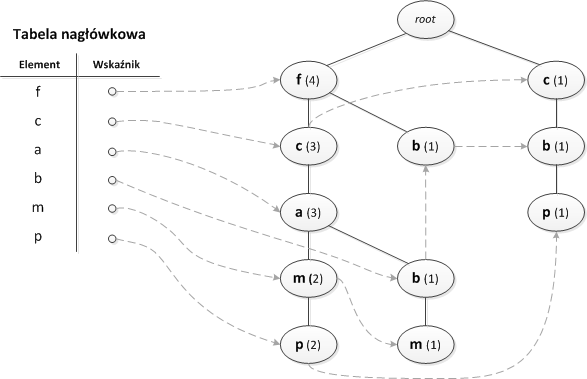
\includegraphics{figures/02/fptree.png}
\caption{Ilustracja przykładowego FP-drzewa dla zbioru danych z tablicy~\ref{example:fp_data}}\label{rys:fptree}
\end{figure}

\subsubsection{Kompresja bazy danych}
Pierwszy etap polega na znalezieniu wszystkich $1$-zbiorów częstych występujących w bazie danych $DB$. Po ich odnalezieniu ($F_1$ - zbiór znalezionych $1$-zbiorów częstych) z każdej transakcji $T$ usuwany jest ten element, który nie należy do $F_1$. 

W wyniku usunięcia elementów nie tworzących jednoelementowych zbiorów częstych, baza ma zazwyczaj znacznie mniejszy rozmiar niż wyjściowa baza danych. Dodatkowo w tym kroku elementy w każdej transakcji zostają posortowane według malejącej wartości ich wsparcia.

\subsubsection{Konstrukcja FP-drzewa}\label{fptree:construction}
\begin{alg}\label{alg:fptre:econstruction}
	\emph{Konstrukcja FP-drzewa}.

	\textbf{Input:} Baza danych transakcji $DB$ oraz minimalne wsparcie (\id{minsup}).

	\textbf{Output:} FP-drzewo utworzone na podstawie zawartości $DB$

	\textbf{Metoda:} Poniżej zostanie opisany proces konstrukcji FP-drzewa.

	\begin{enumerate}
		\item Przeskanowanie bazy danych transakcji $DB$ odbywa się jednokrotnie. Utworzony na tej podstawie zostanie zbiór $F$, zawierający 1-zbiory częste. Posortowany malejąco zbiór $F$ na podstawie wartości $support$ dla każdego elementu tworzy listę $FList$, czyli listę wszystkich elementów tworzących jednoelementowe zbiory częste.
		\item Tworzony jest pierwszy element drzewa - korzeniem zostaje (zgodnie z definicją~\ref{fptree:def}) element z etykietą \id{null}. Dla każdej transakcji w bazie danych $DB$ wykonywane jest, co następuje.
		\begin{quote}
			Wybierane są elementy częste z transakcji, a następnie sortowane zgodnie z kolejnością w $FList$. Niech taka posortowana lista elementów częstych ma postać $[p|P]$, gdzie $p$ jest pierwszym elementem, a \id{P} jest pozostałą częscią listy. Następnie wywoływana jest funkcja $insertTree([p|P], T)$, gdzie \id{T} jest FP-drzewem.
		\end{quote}
			\paragraph{Funkcja insertTree} Jeśli drzewo \id{T} ma dziecko \id{N} takie, że $N.itemName = p.itemName$, zwiększana jest wartość $N.count$ o wartość 1; w przeciwnym wypadku tworzony jest nowe element \id{N} z wartością $count = 1$, a wskaźnik rodzica ustawiany jest na \id{T} oraz wskaźnik sąsiedzctwa elementu ustawiany jest na element z takim samym $itemName$. Jeśli lista \id{P} była niepusta, to wywoływana jest funkcja $insertTree(P, T)$ rekurencyjnie, w przeciwnym wypadku kończone jest działanie funkcji.
	\end{enumerate}
\end{alg}

\subsubsection{Eksploracja FP-drzewa}
Po utworzeniu FP-drzewa przeprowadzana jest jego analiza w celu znalezienia wszystkich zbiorów częstych. Eksploracja bazuje na obserwacji, że dla każdego $1$-zbioru częstego $\alpha$ wszystkie częste nadzbiory tego zbioru są reprezentowane w FP-drzewie przez ścieżki zawierające wierzchołek (bądź wierzchołki) $\alpha$.

Analiza rozpoczyna się od znalezienia dla każdego $1$-zbioru częstego $\alpha$ wszystkich ścieżek w FP-drzewie, których końcowym wierzchołkiem jest wierzchołek odpowiadający zbiorowi $\alpha$. Pojedyncza ścieżka, na której końcu znajduje się wierzchołek $\alpha$ w dalszej analizie będzie nazywana \emph{ścieżką prefiksową wzorca} $\alpha$.

Poniżej zaprezentowany zostanie pseudokod algorytmu przeszukiwania FP-drzewa celem odnalezienia reguł asocjacyjnych.

\begin{alg}
	\emph{FP-growth: Przeszukiwanie FP-drzewa celem odnalezienia reguł asocjacyjnych}.

	\textbf{Input:} Baza danych transakcji $DB$ reprezentowana przez FP-drzewo zwrócone przez algorytm~\ref{alg:fptre:econstruction} oraz minimalne wsparcie (\id{minsup}).

	\textbf{Output:} Kompletny zbiór reguł asocjacyjnych.

	\textbf{Metoda:} Wywołanie \proc{FP-growth}$(FP-drzewo, null)$.

	
\begin{codebox}
	\Procname{$\proc{FP-growth}$(\id{Tree}, $\alpha$)}
		\li \If $\id{Tree}$ zawiera jedną ścieżkę prefiksową
			\li \Then
				\id{P} $\gets$ ścieżka prefiksowa drzewa \id{Tree}
				\li \id{Q} $\gets$ wieloczęściowa ścieżka z najwyższym elementem zastąpionym przez korzeń $null$
					\li \For \textbf{each} kombinacja ($\beta$) elementów z \id{P}
						\li \Do
							\textbf{generuj} regułę $\beta \cup \alpha$ z $support =$ minimalna wartość $support$ elementów w $\beta$
							\li niech $freqPatternSet(\id{P})$ będzie zbiorem wygenerowanych do tej pory reguł
						\End
			\li \Else 
				\id{Q} $\gets$ \id{Tree}
				\li \For \textbf{each} element $a_i \in \id{Q}$
					\li \Do
					\textbf{generuj} regułę $\beta \gets a_i \cup \alpha$ z $support = a_i.support$
					\li \textbf{stwórz} warunkową bazę wzorców z $\beta$ oraz FP-drzewo ($Tree_{\beta}$) dla $\beta$
						\li	\If $Tree_{\beta} \neq \emptyset$
							\li \Then
							\textbf{call} $\proc{FP-growth}$($Tree_{\beta}$, $\beta$)
								\End
							\li niech $freqPatternSet(\id{Q})$ będzie zbiorem wygenerowanych do tej pory reguł
						\End
				\End
		\li \textbf{return} $freqPatternSet(\id{P}) \cup freqPatternSet(\id{Q}) \cup (freqPatternSet(\id{P}) \times freqPatternSet(\id{Q}))$
		\End
\end{codebox}
\end{alg}

\subsubsection{Przykład eksploracji FP-drzewa}
W rozdziale pt.~\emph{\nameref{sec:example_fptree}} zaprezentowano sposób budowy FP-drzewa. Opierając się na przykładzie wprowadzonym w tablicy~\ref{example:fp_data} przedstawiony zostanie przykład działania eksploracji zbudowanego na tej podstawie FP-drzewa, które zostało zaprezentowane na rysunku~\ref{rys:fptree}.

Przykład należy rozpocząć od spostrzeżenia, że wszystkie reguły asocjacyjne, zawierające element częsty $a_i$ mogą być zebrane poprzez wyjście ze wskaźnika z tablicy nagłówkowej FP-drzewa, a następnie podążając zgodnie z kolejnymi wskaźnikami na wystąpienia danego elementu w drzewie. W przykładzie analiza zostanie przeprowadzona od końca - tj. podąrzając od elementu najmniej licznego spośród elementów częstych.

Dla elementu $p$ regułą częstą jest $p: 3$, która posiada dwie ścieżki w drzewie: $\langle f: 4, c: 3,$ $a: 3, m: 2, p: 2\rangle$ oraz $\langle c: 1, b: 1, p: 1\rangle$. Pierwsza ścieżka oznacza, że wartość ''$( f, c, a, m, p )$'' występuje w bazie danych $DB$ dwukrotnie. Warto zauważyć, że pierwsza ścieżka oznacza również, że ciąg ''$( f, c, a )$'' występuje w bazie dwukrotnie, a ''$(f)$'' nawet czterokrotnie. Jednakże występują one jednocześnie z $p$ jedynie dwukrotnie. Dlatego też, do analizy wartości występujących razem z $p$ tylko ścieżka prefiksowana $\langle f: 2, c: 2, a: 2, m: 2\rangle$ (lub zapisane krócej: $\langle fcam: 2\rangle$) jest brana pod uwagę. Podobnie w przypadku drugiej ścieżki - wynika z niej, że ciąg ''$(c, b, p)$'' występuje tylko raz w transakcjach w bazie danych $DB$, lub też prefiksowana ścieżka dla $p$ ma postać $\langle cb: 1 \rangle$. Te dwie ścieżki prefiksowane elementu $p$ ( czyli $\lbrace ( fcam: 2 ), (cb: 1) \rbrace$) tworzą bazę wzorca elementu $p$ (\english{subpattern-base}), która jest nazywana \emph{warunkową bazę wzorców} z $p$ (\english{conditional pattern base}) - to znaczy bazę wzorca pod warunkiem występowania elementu $p$~\cite{Main:FPgrowth}. Konstrukcja FP-drzewa na tej warunkowej bazie wzorców (które nazywane jest \emph{warunkowym FP-drzewem} elementu $p$ \english{conditional FP-tree}) prowadzi tylko do jednej gałęzi - $(c:3)$. Stąd też tylko jeden wzorzeć jest dziedziczony - $(cp:4)$. (Warto zauważyć, że wzorzec jest zbiorem elementów, który jest reprezentowany przez ciąg.) Poszukiwanie częstych wzorców związanych z elementem $p$ kończy działanie.

Dla wierzchołka $m$ jego bezpośrednim wzorcem częstym jest $(m:3)$, posiada on również dwie ścieżki: $\langle f: 4, c: 3, a: 3, m: 2 \rangle$ oraz $\langle f: 4, c: 3, a: 3, b: 1, m: 1 \rangle$. W obu tych ścieżkach można zauważyć, że $m$ występuje razem z $p$, jednakże $p$ w tym miejscu nie musi być brane pod uwagę, ponieważ wszystkie wzorce częste dla tego elementu zostały znalezione wcześniej (opisano to akapit wcześniej). Wykonując działania podobnie, jak w poprzednim akapicie wyznaczona zostanie warunkowa baza wzorców o postaci $\lbrace (fca: 2), (fcab: 1) \rbrace$. Skonstruowane na tej podstawie FP-drzewo, czyli warunkowe FP-drzewo elementu $m$ ($\langle f: 3, c: 3, a: 3 \rangle$) posiada jedną ścieżkę częstą, co można zaobserwować na rysunku~\ref{rys:mining_fptree}. Następnie przeprowadzona jest rekurencyjna eksploracja tego warunkowego drzewa poprzez wywołanie $mine(\langle f: 3, c: 3, a: 3 \rangle | m)$.

\begin{figure}[h]
\centering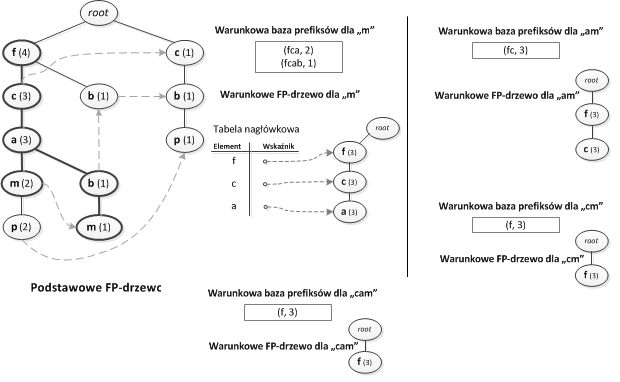
\includegraphics{figures/02/mining_fptree.png}
\caption{Eksploracja warunkowego FP-drzewa dla elementu $m$ (FP-tree $| m$)~\cite{Main:FPgrowth}}\label{rys:mining_fptree}
\end{figure}

Rysunek~\ref{rys:mining_fptree} ilustruje, że wywołanie $mine(\langle f: 3, c: 3, a: 3 \rangle | m)$ poddaje przetwarzaniu trzy elementy: $(a), (c), (f)$ sekwencyjnie. Przetwarzanie pierwszego tworzy częsty wzorzec o postaci $(am: 3)$, warunkową bazę wzorców $\lbrace (fc: 3) \rbrace$, a następnie wywoływana jest funkcja $mine(\langle f: 3, c: 3 \rangle | am)$; kolejny tworzy częsty wzorzec o postaci $(cm: 3)$, warunkową bazę wzorców $\lbrace (f: 3)\rbrace$, a następnie wywoływana jest funkcja $mine(\langle f: 3 \rangle | cm)$; trzecie natomiast tworzy jedynie częsty wzorzec $(fm: 3)$. Dalsze wywołanie metody $mine(\langle f: 3, c: 3 \rangle | am)$ tworzy dwa wzorce $(cam: 3)$ oraz $(fam: 3)$, warunkową bazę wzorców $\lbrace ( f: 3 ) \rbrace$, która prowadzi do wywołania $mine(\langle f: 3 \rangle | cam)$, czego wynikiem jest najdłuższy wzorzec częsty $(fcam: 3)$. Podobnie, wywołanie $mine(\langle f: 3 \rangle | cm)$ tworzy jednen wzorzec $(fcm: 3)$. 

Z przeprowadzonej analizy wynika, że zbiór wszystkich wzorców częstych zawierający $m$ ma postać $\lbrace (m: 3), (am: 3), (cm: 3), (fm: 3), (cam: 3), (fam: 3), (fcam: 3), (fcm: 3) \rbrace$. Wynika z tego, że jedna ścieżka w FP-drzewie może być przeanalizowana poprzez wygenerowanie wszystkich kombinacji (bez powtórzeń) elementów na tej ścieżce.

Podobnie, $b$ tworzy $(b: 3)$, posiada również trzy ścieżki: $\langle f:4, c:3, a:3, b:1 \rangle$, $\langle f:4, b:1 \rangle$ oraz $\langle c:1, b:1 \rangle$. Ponieważ warunkowa baza wzorca tego elementu $\lbrace (fca:1), (f:1), (c:1)\rbrace$ nie generuje żadnych elementów częstych, eksploracja po elemencie $b$ kończy działanie. 

Element $a$ tworzy jeden element częsty $(a:3)$ oraz bazę wzorca $\lbrace (fc:3) \rbrace$, czyli FP-drzewo posiadające jedną ścieżkę. Wynika z tego, że zbiór częstych wzorców może być wygenerowany poprzez wygenerowanie wszystkich ich kombinacji. Dokonując konkatenacji z $(a:3)$, otrzymany zostanie zbiór $\lbrace (fa:3), (ca:3), (fca:3) \rbrace$. Wierzchołek $c$ generuje $(c:4)$, a także bazę wzorca $\lbrace (f:3) \rbrace$, a zbiór częstych wzorców skojarzonych z $(c:3)$ ma zawartość $\lbrace (fc:3)\rbrace$. Analiza elementu $f$ tworzy jedynie $(f:4)$, lecz bez warunkowych baz wzorców.

\begin{table}
	\centering
	\begin{tabular}{|c|c|c|} \hline
	\textbf{Element} &  \textbf{Warunkowa baza wzorców} & \textbf{Warunkowe FP-drzewo} \\ \hline
	$p$ & $\lbrace ( fcam: 2 ), (cb: 1) \rbrace$ & $\lbrace (c:3) \rbrace | p$ \\ 
	$m$ & $\lbrace ( fca: 2 ), (fcab: 1) \rbrace$ & $\lbrace (f:3, c:3, a:3) \rbrace | m$ \\ 
	$b$ & $\lbrace ( fca: 2 ), (f: 1), (c: 1) \rbrace$ & $\emptyset$ \\ 
	$a$ & $\lbrace ( fc: 3 ) \rbrace$ & $\lbrace (f:3, c:3) \rbrace | a$ \\ 
	$c$ & $\lbrace ( f: 3 ) \rbrace$ & $\lbrace (f:3) \rbrace | c$ \\ 
	$f$ & $\emptyset$ & $\emptyset$ \\ \hline
	\end{tabular}
	\caption{Wyniki eksploracji FP-drzewa dla przykładu opartego na danych w tablicy~\ref{example:fp_data}\label{example:sum_patterns}}
\end{table}

W tablicy~\ref{example:sum_patterns} zebrane zostały baze wzorców oraz warunkowe FP-drzewa dla poszczególnych elementów.
%
\chapter{Rozwinięcie}

Rozdziały dokumentujące pracę własną studenta: opisujące ideę, sposób lub metodę 
rozwiązania postawionego problemu oraz rozdziały opisujące techniczną stronę rozwiązania 
--- dokumentacja techniczna, przeprowadzone testy, badania i uzyskane wyniki. 

Praca musi zawierać elementy pracy własnej autora adekwatne do jego wiedzy praktycznej uzyskanej w
okresie studiów. Za pracę własną autora można uznać np.: stworzenie aplikacji informatycznej lub jej
fragmentu, zaproponowanie algorytmu rozwiązania problemu szczegółowego, przedstawienie projektu 
np.~systemu informatycznego lub sieci komputerowej, analizę i ocenę nowych technologii lub rozwiązań
informatycznych wykorzystywanych w przedsiębiorstwach, itp. 

Autor powinien zadbać o właściwą dokumentację pracy własnej obejmującą specyfikację założeń i 
sposób realizacji poszczególnych zadań
wraz z ich oceną i opisem napotkanych problemów. W przypadku prac o charakterze 
projektowo-implementacyjnym, ta część pracy jest zastępowana dokumentacją techniczną i użytkową systemu. 

W pracy \textbf{nie należy zamieszczać całego kodu źródłowego} opracowanych programów. Kod źródłowy napisanych
programów, wszelkie oprogramowanie wytworzone i wykorzystane w pracy, wyniki przeprowadzonych
eksperymentów powinny być umieszczone na płycie CD, stanowiącej dodatek do pracy.

\section*{Styl tekstu}

Należy\footnote{Uwagi o stylu pochodzą częściowo ze stron Macieja Drozdowskiego~\cite{mdro}.} 
stosować formę bezosobową, tj.~\emph{w pracy rozważono ......, 
w ramach pracy zaprojektowano ....}, a nie: \emph{w pracy rozważyłem, w ramach pracy zaprojektowałem}. 
Odwołania do wcześniejszych fragmentów tekstu powinny mieć następującą postać: ,,Jak wspomniano wcześniej, ....'', 
,,Jak wykazano powyżej ....''. Należy unikać długich zdań. 

,,Ilość'' i ,,liczba''. Proszę zauważyć, liczba dotyczy rzeczy policzalnych, np.~liczba osób, liczba zadań, procesorów. 
Ilość dotyczy rzeczy niepoliczalnych, np.~ilość wody, energii. Należy starać się wyrażać precyzyjnie, tj.~zgodnie 
z naturą liczonych obiektów.\footnote{(DW) Według wytycznych Rady Języka Polskiego obie formy są dopuszczalne
zarówno do obiektów policzalnych, jak i niepoliczalnych. W tekstach technicznych warto być jednak precyzyjnym.}

Niedopuszczalne są zwroty używane w języku potocznym. W pracy należy używać terminologii informatycznej, która ma 
sprecyzowaną treść i znaczenie. Nie należy używać ,,gazetowych'' określeń typu: 
silnik bazy danych, silnik programu, maszyna skryptowa, elektroniczny mechanizm, mapowanie, string, gdyż nie wiadomo 
co one właściwie oznaczają. 

Niedopuszczalne jest pisanie pracy metodą \emph{cut\&paste}, bo jest to plagiat i dowód intelektualnej indolencji autora.
Dane zagadnienie należy opisać własnymi słowami. Zawsze trzeba powołać się na zewnętrzne źródła. 


%
\chapter{Zakończenie}

Zakończenie pracy zwane również Uwagami końcowymi lub Podsumowaniem powinno zawierać ustosunkowanie
się autora do zadań wskazanych we wstępie do pracy, a w szczególności do celu i zakresu pracy oraz
porównanie ich z faktycznymi wynikami pracy. Podejście takie umożliwia jasne określenie stopnia
realizacji założonych celów oraz zwrócenie uwagi na wyniki osiągnięte przez autora w ramach jego
samodzielnej pracy.

Integralną częścią pracy są również dodatki, aneksy i załączniki np.~płyty CDROM
zawierające stworzone w ramach pracy programy, aplikacje i projekty.


% All appendices and extra material, if you have any.
%\cleardoublepage\appendix%
%
\chapter{Parę słów o stylu \texttt{ppfcmthesis}}

\section{Różnice w stosunku do ,,oficjalnych'' zasad składu ze stron FCMu}

Autor niniejszego stylu nie zgadza się z niektórymi zasadami wprowadzonymi w oficjalnym 
dokumencie FCMu.\footnote{\url{http://www.fcm.put.poznan.pl/platon/dokumenty/dlaStudentow/egzaminDyplomowy/zasadyRedakcji}}
Poniższe elementy są składane nieco inaczej w stosunku do ,,oficjalnych'' wytycznych.

\begin{itemize}
    \item Promotor na stronie tytułowej jest umiejscowiony w centralnej osi pionowej strony (a
    nie po prawej stronie).
    
    \item Czcionka użyta do składu to nie Times New Roman.
    
    \item Spacje między tytułami akapitów oraz wcięcia zostały pozostawione takie, jak są zdefiniowane
    oryginalnie w pakiecie Memoir (oraz w \LaTeX{}u). Jeśli zdefiniowano ,,polską'' opcję składu,
    to będzie w użyciu wcięcie pierwszego akapitu po tytułach rozdziałów. Przy składzie ,,angielskim''
    tego wcięcia nie ma.

    \item Odwrócona jest kolejność rozdziałów \emph{Literatura} i \emph{Dodatki}.

    \item Na ostatniej stronie umieszczono stopkę informującą o prawach autorskich i programie
    użytym do składu.
    
    \item Nie do końca zgadzam się ze stwierdzeniem, iż ,,zamieszczanie list tabel, rysunków, 
    wykresów w pracy dyplomowej jest nieuzasadnione''. Niektóre typy publikacji zawierają tabele i rysunki, których
    skorowidz umożliwia łatwiejsze ich odszukanie. Ale niech będzie.

    \item Styl podpisów tabel jest taki sam, jak rysunków i odmienny od FCMowego. 
    Jeśli ktoś koniecznie chce mieć zgodne z wytycznymi
    podpisy, to zamiast \texttt{caption} niech użyje \texttt{fcmtcaption} do podpisywania tablic oraz
    \texttt{fcmfcaption} do podpisywania rysunków. Podpisy pod rysunkami pozostaną pełne, a nie skrócone (,,Rys.'').
    
    \item Styl formatowania literatury jest nieco inny niż proponowany przez FCM.
\end{itemize}


%
\chapter{Składanie dokumentu w systemie \LaTeX}

Po pierwsze to gratulacje --- dobry wybór. W tym rozdziale znajduje się
garść informacji o tym, jak poprawnie składać tekst pracy w systemie \LaTeX{} wraz z 
przykładami, które mają służyć do przeklejania do własnych dokumentów.

\section{Narzędzia}
Pracując pod systemem Windows, polecam:
\begin{itemize}
    \item MikTeX, \url{http://www.miktex.org/},
    \item JEdit, \url{http://www.jedit.org/},
    \item TeXlipse, \url{http://texlipse.sourceforge.net/},
    \item Kile, \url{http://kile.sourceforge.net/},
    \item Ghostview, Ghostscript (podgląd dokumentów PDF bez blokowania pliku):\\
        \url{http://www.cs.wisc.edu/~ghost/}. 
\end{itemize}

Po zainstalowaniu tych narzędzi wystarczy wykonać polecenie \texttt{compile.bat} (który
jest skryptem wsadowym dla Windows). Dla tych, którzy wolą nieco automatyzacji --- skrypt
\texttt{latexmk}, który jest w MikTeXu (a który potrzebuje zainstalowanego Perla) jest
również bardzo wygodny: \texttt{latexmk -pdf -pvc main.tex}.

\section{Edycja tekstu}
\chaptermark{Tytuł rozdziału, jeśli pełen się nie mieści\ldots{}}{}

\subsection{Struktura dokumentu}

Praca składa się z rozdziałów (\texttt{chapter}) i podrozdziałów (\texttt{section}).
Ewentualnie można również rozdziały zagnieżdzać (\texttt{subsection}, \texttt{subsubsection}),
jednak nie powinno się wykraczać poza drugi poziom hierarchii (czyli \texttt{subsubsection}).

\subsection{Akapity i znaki specjalne}

Każdy akapit to po prostu blok tekstu. Nieważne jak sformatowany --- to zrobi już
system $\LaTeX$.

Akapity rozdziela się od siebie przynajmniej jedną pustą linią. Podstawowe
instrukcje, które się przydają to \emph{wyróżnienie pewnych słów}. Można również
stosować \textbf{styl pogrubiony}, choć nie jest to generalnie zalecane.

Należy pamiętać o zasadach polskiej interpunkcji i ortografii. Po spójnikach 
jednoliterowych warto wstawić znak tyldy ($\sim$), który jest tak zwaną
,,twardą spacją'' i powoduje, że wyrazy nią połączone nie będą rozdzielane
na dwie linie tekstu.

Polskie znaki interpunkcyjne różnią się nieco od angielskich: to jest ,,polski'', a to jest
``angielski''. W kodzie źródłowym tego tekstu będzie widać różnicę.

Proszę również zwrócić uwagę na znak myślnika, który może być pauzą ,,---'' lub
półpauzą: ,,--''. Należy stosować je konsekwentnie. Do łączenia wyrazów używamy
zwykłego ,,-'' (\emph{północno-wschodni}), do myślników --- pauzy lub półpauzy.
Inne zasady interpunkcji i typografii można znaleźć w słownikach.

\subsection{Wypunktowania}

Wypunktowanie z cyframi:
\begin{enumerate}
    \item to jest punkt,
    \item i to jest punkt,
    \item a to jest ostatni punkt.
\end{enumerate}

\noindent
Po wypunktowaniach czasem nie warto wstawiać wcięcia akapitowego. Wtedy przydatne jest
polecenie \texttt{noindent}. Wypunktowanie z kropkami (tzw.~\emph{bullet list}) wygląda tak:
\begin{itemize}
    \item to jest punkt,
    \item i to jest punkt,
    \item a to jest ostatni punkt.
\end{itemize}

\noindent
Wypunktowania opisowe właściwie niewiele się różnią:
\begin{description}
    \item[elementA] to jest opis,
    \item[elementB] i to jest opis,
    \item[elementC] a to jest ostatni opis.
\end{description}


\subsection{Polecenia pakietu \texttt{ppfcmthesis}}

Parę poleceń zostało zdefiniowanych aby uspójnić styl pracy. Są one przedstawione poniżej
(oczywiście nie trzeba się do nich stosować).

\paragraph{Makra zdefiniowane dla języka angielskiego.} Są nimi: \texttt{termdef} oraz \texttt{acronym}.
Przykłady poniżej obrazują ich przewidywane użycie w tekście.
\begin{center}\footnotesize%
\begin{tabular}{l >{\rightskip\fill}p{12cm}}
\toprule
źródło   & \texttt{we call this a $\backslash$termdef\{Database Management System\} ($\backslash$acronym\{DBMS\})} \\ \cmidrule(lr){2-2}
docelowo & we call this a \termdef{Database Management System} (\acronym{DBMS}) \\ 
\bottomrule
\end{tabular}
\end{center}

\paragraph{Makra zdefiniowane dla języka polskiego.} Podobnie jak dla języka angielskiego zdefiniowano
odpowiedniki polskie: \texttt{defini\-cja}, \texttt{akronim} oraz \texttt{english} dla tłumaczeń angielskich
terminów. Przykłady poniżej obrazują ich przewidywane użycie w tekście.
\begin{center}\footnotesize%
\begin{tabular}{l >{\rightskip\fill}p{12cm}}
\toprule
źródło   & \texttt{nazywamy go $\backslash$definicja\{systemem zarządzania bazą danych\} ($\backslash$akronim\{DBMS\}, $\backslash$english\{Database Management System\})} \\ \cmidrule(lr){2-2}
docelowo & nazywamy go \definicja{systemem zarządzania bazą danych} (\akronim{DBMS}, \english{Database Management System}) \\ \bottomrule
\end{tabular}
\end{center}


\subsection{Rysunki}

Format wstawianych rysunków zależy od tego czy używa się do kompilacji polecenia
\texttt{latex}, czy też \texttt{pdflatex}. Oba powinny dać dokładnie ten sam wynik końcowy,
ale praca z nimi jest nieco inna.

\begin{description}
    \item[latex] To polecenie kompiluje źródła \LaTeX{}owe do pliku 
        z rozszerzeniem \texttt{dvi}. Ten plik można przeglądać przy pomocy specjalizowanych programów
        takich jak przykładowo Yap obecny z dystrybucją Mik\TeX{}a. Aby uzyskać docelowy plik \akronim{PDF}
        należy przekonwertować plik \texttt{dvi} przy pomocy programu \texttt{dvipdfm}. 
        
        \textbf{UWAGA:} korzystając z programu \texttt{latex}, wszystkie rysunki muszą być w formacie \akronim{EPS}
        (\english{encapsulated postscript}).

    \item[pdflatex] To polecenie kompiluje źródła \LaTeX{}owe bezpośrednio do pliku \akronim{PDF}.
    
        \textbf{UWAGA:} korzystając z programu \texttt{pdflatex}, wszystkie rysunki muszą być w formacie \akronim{PDF},
        \akronim{JPG} lub \akronim{PNG}.
\end{description}

Można oczywiście używać obu systemów --- wtedy pliki rysunków muszą po prostu być dostępne w obu formatach.

Wszystkie rysunki (w tym również diagramy, szkice i inne) osadzamy w środowisku 
\texttt{figure} i umieszczamy podpis \emph{pod} rysunkiem, w formie elementu \texttt{caption}. Rysunki powinny
zostać umieszczone u góry strony (osadzone bezpośrednio w treści strony zwykle utrudniają czytanie tekstu).
Rysunek~\ref{rys:plama} zawiera przykład pełnego osadzenia rysunku na stronie.

\begin{figure}[t] % możliwe opcje to 't' - top, 'b' - bottom, 'h' - 'here', ale zaleca się 't'
\centering
\includegraphics[width=5cm]{figures/template/logo-pp}
\caption{Logo Politechniki Poznańskiej.}\label{rys:plama}
\end{figure}

\begin{figure}[t]
\centering
\includegraphics[width=5cm]{figures/template/logo-pp}
\fcmfcaption{Logo Politechniki Poznańskiej. Formatowanie zgodne z wytycznymi FCMu.}\label{rys:plama2}
\end{figure}

Zasady FCMu sugerują nieco inne nagłówki rysunków. Dostepne są one poleceniem \texttt{fcmfcaption} (zob.~rysunek
\ref{rys:plama2}), jeśli ktoś woli mieć podpisy niespójne z rysunkami\ldots

\subsection{Tablice}

Tablice to piękna rzecz, choć akurat ich umiejętne tworzenie w \LaTeX{}u nie jest łatwe. 
Jeśli tablica jest skomplikowana, to pewnie łatwiej będzie ją wykonać w programie
OpenOffice, a następnie wyeksportować jako plik \akronim{PDF}. W każdym przypadku tablice wstawia się podobnie
jak rysunki, tylko że w środowisko \texttt{table}. Tradycja typograficzna sugeruje umieszczenie opisu tablicy, a więc
elementu \texttt{caption} ponad jej treścią (inaczej niż przy rysunkach).  

Tablica~\ref{tab:tabela} pokazuje pełen przykład.

\begin{table}[h]
\caption{Przykładowa tabela. Styl opisu jest zgodny z rysunkami.}\label{tab:tabela}
\centering\footnotesize%
\begin{tabular}{l c}
\toprule
artykuł & cena [zł] \\
\midrule
bułka   & $0,4$ \\
masło   & $2,5$ \\
\bottomrule
\end{tabular}
\end{table}

Zasady FCMu sugerują nieco inne nagłówki tablic. Dostepne są one poleceniem \texttt{fcmtcaption} (zob.~tablicę
\ref{tab:tabela2}), jeśli ktoś woli mieć podpisy niespójne z rysunkami\ldots

\begin{table}[h]
\fcmtcaption{Przykładowa tabela. Styl opisu jest zgodny z wytycznymi FCMu.}\label{tab:tabela2}
\centering\footnotesize%
\begin{tabular}{l c}
\toprule
artykuł & cena [zł] \\
\midrule
bułka   & $0,4$ \\
masło   & $2,5$ \\
\bottomrule
\end{tabular}
\end{table}


\subsection{Checklista}

W katalogu źródeł stylu \texttt{ppfcmthesis} znajduje się plik \texttt{CHECKLIST} --- należy
sprawdzić, czy nie popełniło się któregoś z wymienionych tam błędów.


\section{Literatura i materiały dodatkowe}

Materiałów jest mnóstwo. Oto parę z nich:
\begin{itemize}
    \item \emph{The Not So Short Introduction\ldots}, która posiada również tłumaczenie 
    w języku polskim.\\
    \url{http://www.ctan.org/tex-archive/info/lshort/english/lshort.pdf}

    \item Klasy stylu \texttt{memoir} posiadają bardzo wiele informacji o składzie tekstów
    anglosaskich oraz sposoby dostosowania \LaTeX{}a do własnych potrzeb.\\
    \url{http://www.ctan.org/tex-archive/macros/latex/contrib/memoir/memman.pdf}
    
    \item Nasza grupa dyskusyjna i repozytorium SVN są również dobrym miejscem aby zapytać
    (lub sprawdzić czy pytanie nie zostało już zadane).\\
    \url{https://ophelia.cs.put.poznan.pl/svn/put-latex/trunk}

    \item Dla łaknących więcej wiedzy o systemie \LaTeX{} podstawowym źródłem informacji
    jest książka Lamporta~\cite{Lamport:LDP85}. Prawdziwy \emph{hardcore} to oczywiście
    \emph{The \TeX{}book} profesora Knutha~\cite{Knuth:ct-a}.
\end{itemize}



% Bibliography (books, articles) starts here.
\bibliographystyle{plalpha}{\raggedright\sloppy\small\bibliography{bibliography}}

% Colophon is a place where you should let others know about copyrights etc.
\ppcolophon

\end{document}
